\section{ÁP SUẤT - ĐỘNG NĂNG CỦA CHẤT KHÍ THEO MÔ HÌNH ĐỘNG HỌC PHÂN TỬ}
\subsection{LÝ THUYẾT TRỌNG TÂM}
\subsubsection{Áp suất chất khí theo mô hình động học phân tử}
\begin{boxdl}
	Áp suất khí tác dụng lên thành bình càng tăng khi các phân tử khí chuyển động nhiệt càng nhanh, khối lượng và mật độ phân tử khí càng lớn.\\
	Biểu thức áp suất chất khí tác dụng lên thành bình:
	\begin{equation}
		p=\dfrac{1}{3}\mu m\overline{v^2}
	\end{equation}
\end{boxdl}
Trong đó:
\begin{itemize}
	\item $p$: áp suất khí, đơn vị trong hệ SI là $\si{\pascal}$;
	\item $m$: khối lượng của mỗi phân tử khí, đơn vị trong hệ SI là $\si{\kilogram}$;
	\item $\mu$: mật độ phân tử khí, đơn vị trong hệ SI là $\si{\meter^{-3}}$;
	\item $\overline{v^2}$: trung bình của bình phương tốc độ chuyển động nhiệt của mỗi phân tử khí, đơn vị trong hệ SI là $\si{\meter^2/\second^2}$.
\end{itemize}
\begin{luuy}
	Căn bậc hai của $\overline{v^2}$ là $\sqrt{\overline{v^2}}$, độ lớn của đại lượng này không phải là tốc độ trung bình của các phân tử. Nó được gọi là \textit{tốc độ căn quân phương} của phân tử.
\end{luuy}
\subsubsection{Động năng tịnh tiến trung bình của phân tử khí}
\begin{boxdl}
	Động năng tịnh tiến trung bình của phân tử khí tỉ lệ với nhiệt độ tuyệt đối của khí:
	\begin{equation}
		W_\text{đ}=\dfrac{3}{2}kT
	\end{equation}
	
\end{boxdl}
\begin{boxdn}
	Trong đó, hằng số Boltzmann $k$ là hằng số khí đặc trưng cho mối liên hệ giữa nhiệt độ và năng lượng. Giá trị của hằng số Boltzmann trong hệ SI bằng
	$$k=\dfrac{R}{N_A}\approx\SI{1.38E-23}{\joule/\kelvin}.$$
\end{boxdn}

\begin{boxkn}
	Có thể biểu diễn sự phụ thuộc của áp suất theo nhiệt độ tuyệt đối $T$ và mật độ phân tử khí $n$:
	$$pV=\dfrac{N}{N_\text{A}}RT\Rightarrow p=\dfrac{N}{V}\cdot\dfrac{R}{N_\text{A}}\cdot T=\mu kT.$$
	Hay
	$$p=\dfrac{2}{3}\mu W_\text{đ}.$$
\end{boxkn}
\subsection{VÍ DỤ MINH HOẠ}
\begin{dang}{Giải thích được chuyển động của các phân tử ảnh hưởng như thế nào đến áp suất tác dụng lên thành bình và từ đó rút ra được hệ thức $p=\dfrac{1}{3}\mu m\overline{v^2}$}
	\end{dang}
\begin{vd}
	Trong bài tập này, chúng ta sẽ chứng minh lại những điều được học trong phần lý thuyết.
		\begin{enumerate}[label=\alph*)]
			\item Em hãy giải thích vì sao áp suất do các phân tử khí tác dụng lên thành bình phụ thuộc vào tốc độ chuyển động nhiệt, khối lượng và mật độ của các phân tử khí?
			\item Bây giờ, ta xét mô hình va chạm một chiều đơn giản: Hệ gồm các phân tử khí khối lượng $m$ chuyển động dọc theo trục $Ox$ với tốc độ $v_x$ đến va chạm đàn hồi với thành bình rồi bật ngược trở lại với cùng tốc độ ban đầu. Trong thời gian va chạm $\Delta t$, số phân tử đập vào diện tích $S$ của thành bình là số phân tử chứa trong một hình trụ đáy $S$, chiều cao $h=v_x\Delta t$. 
			\begin{center}
				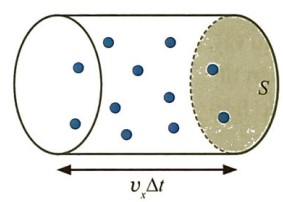
\includegraphics[width=0.3\linewidth]{figs/VN12-Y24-PH-SYL-014-1}
				\captionof{figure}{Minh hoạ về các phân tử khí đập vào thành bình trong thời gian $\Delta t$}
			\end{center}
			Gọi $\mu$ là mật độ phân tử khí. Xác định áp suất do các phân tử khí tác dụng lên thành bình theo $m$, $v_x$, $\mu$.
			\item Thực tế, các phân tử khí chuyển động hỗn loạn không có phương nào ưu tiên. Từ kết quả thu được ở câu b, em hãy mở rộng cho trường hợp chuyển động 3 chiều.
		\end{enumerate}
\loigiai{\begin{enumerate}[label=\alph*)]
				\item Khi các phân tử khí chuyển động nhiệt đến va chạm vào thành bình sẽ gây ra áp suất lên thành bình. Áp suất này được tính bằng áp lực của các phân tử khí lên một đơn vị diện tích thành bình.\\
				Áp lực này càng lớn khi
				\begin{itemize}
					\item động lượng trước va chạm $m\vec{v}$ của các phân tử khí càng lớn $\Leftrightarrow m$ và $v$ càng lớn;
					\item số lượng phân tử khí va chạm với thành bình sau mỗi giây càng lớn $\Leftrightarrow$ mật độ phân tử khí $n$ càng lớn.
				\end{itemize}
				\item Sau khi va chạm với thành bình thì phân tử khí bị bật ngược trở lại với vận tốc $\vec{v}'_x$ với $v'_x=v_x$. Lực do thành bình tác dụng lên mỗi phân tử khí:
				$$\vec{f}_x=\dfrac{\Delta \vec{p}_x}{\Delta t}=\dfrac{m\left(\vec{v}'_x-\vec{v}_x\right)}{\Delta t}\Rightarrow f_x=\dfrac{2mv_x}{\Delta t}.$$
				Trong thời gian va chạm $\Delta t$, số phân tử đập vào diện tích $S$ của thành bình:
				$$N=\mu V=\mu Sv_x\Delta t.$$
				Do $N$ phân tử khí có thể chuyển động dọc trục $Ox$ theo hai chiều ngược nhau nên số lượng trung bình các phân tử khí đến đập vào diện tích $S$ của thành bình theo chiều dương gây áp suất lên thành $S$ là $\dfrac{N}{2}$.\\
				Tổng hợp lực do $\dfrac{N}{2}$ phân tử khí tác dụng lên thành bình theo chiều dương của trục $Ox$:
				$$F_x=\dfrac{N}{2}\cdot f_x=\dfrac{\mu Sv_x\Delta t}{2}\cdot\dfrac{2mv_x}{\Delta t}=\mu mv^2_xS.$$
				Áp suất do các phân tử khí tác dụng lên thành bình:
				$$p=\dfrac{F_x}{S}=\mu mv^2_x.$$
				\item Do phân tử khí chuyển động nhiệt theo cả ba phương và không có phương nào ưu tiên nên $v_x=v_y=v_z$:
				$$v^2=v^2_x+v^2_y+v^2_z=3v^2_x.$$
				Suy ra:
				$$p=\dfrac{1}{3}\mu mv^2.$$
				Vì ta đang xét chuyển động của nhiều phân tử khí nên $v^2$ là giá trị trung bình của bình phương tốc độ chuyển động nhiệt của từng phân tử. Khi đó:
				$$p=\dfrac{1}{3}\mu m\overline{v^2}.$$
			\end{enumerate}
	}
\end{vd}
% ==============================================================
\begin{vd}
	Thực nghiệm đo được tốc độ trung bình của hầu hết các phân tử khí trong khoảng từ vài trăm $\si{\meter/\second}$ đến vài ngàn $\si{\meter/\second}$. Tuy nhiên, phải sau một khoảng thời gian người ta mới cảm nhận được mùi thơm của lọ nước hoa bị đổ trong phòng. Hãy giải thích.
\loigiai{Tốc độ trung bình trên một phương chỉ khoảng $\dfrac{1}{\sqrt{3}}\approx0,58 $ lần tốc độ chuyển động trung bình của phân tử khí. Mặt khác, do sự chuyển hỗn loạn và  trong quá trình khuếch tán, các phân tử nước hoa va chạm với các phân tử khí và các phân tử nước hoa khác làm lệch phương truyền. Do đó, cần nhiều thời gian hơn để các phân tử nước hoa có thể truyền đến được mũi người.
			
	}
\end{vd}
% ====================================================
\begin{vd}
	Tính trung bình bình phương tốc độ trong chuyển động nhiệt của phân tử khí helium có khối lượng mol là $\SI{4}{\gram/\mole}$ ở nhiệt độ $\SI{320}{\kelvin}$. Coi các phân tử khí là giống nhau.
	\loigiai{Áp suất do khí tác dụng lên thành bình:
		\begin{eqnarray}
			&&p=\dfrac{1}{3}\mu m\overline{v^2}\nonumber\\
			&\Leftrightarrow& p=\dfrac{1}{3}\dfrac{N}{V}\cdot m\overline{v^2}\nonumber\\
			&\Leftrightarrow& pV=\dfrac{1}{3}Nm\overline{v^2} \label{eq:14.1}
		\end{eqnarray}
		Mà 
		\begin{equation}
			\label{eq:14.2}\\
			pV=n RT=\dfrac{Nm}{M}RT
		\end{equation}
		Thay (\ref{eq:14.2}) vào (\ref{eq:14.1}):
		$$\overline{v^2}=\dfrac{3RT}{M}=\dfrac{3\cdot\left(\SI{8.31}{\dfrac{\joule}{\mole\cdot\kelvin}}\right)\cdot\left(\SI{320}{\kelvin}\right)}{\SI{4E-3}{\kilogram/\mole}}=\SI{1.99E6}{\meter^2/\second^2}.$$
		
		
	}
\end{vd}
\newpage
\begin{dang}{Vận dụng được biểu thức tính động năng tịnh tiến trung bình của phân tử khí}
\end{dang}
\begin{vd}
	Tính nhiệt độ của một khối khí để động năng tịnh tiến trung bình trong chuyển động tịnh tiến của phân tử khí đó bằng $\SI{1.0}{\electronvolt}$. Lấy $\SI{1}{\electronvolt}=\SI{1.6E-19}{\joule}.$
	\loigiai{Nhiệt độ của khối khí:
			$$T=\dfrac{2}{3}\cdot\dfrac{W_\text{đ}}{k}=\dfrac{2}{3}\cdot\dfrac{\left(\SI{1.6E-19}{\joule}\right)}{\SI{1.38e-23}{\joule/\kelvin}}\approx\SI{7729.5}{\kelvin}.$$
			
	}
\end{vd}
% ==================================================
\begin{vd}
	Xét khối khí chứa trong một bình kín, biết mật độ động năng phân tử (tổng động năng tịnh tiến của các phân tử khí trong $\SI{1}{\meter^3}$ thể tích khí) có giá trị $\SI{E-4}{\joule/\meter^3}$. Tính áp suất của khí trong bình.
\loigiai{Mật độ động năng phân tử:
			$$\varepsilon=\dfrac{NW_\text{đ}}{V}=\mu W_\text{đ}=\SI{E-4}{\joule/\meter^3}.$$
			Áp suất của khí trong bình:
			\begin{align*}
				&p=\dfrac{NRT}{VN_A}=\mu kT\\
				\Rightarrow &p=\dfrac{2}{3}\mu W_\text{đ}=\dfrac{2}{3}\varepsilon=\dfrac{2}{3}\cdot\left(\SI{E-4}{\joule/\meter^3}\right)=\SI{6.67E-5}{\pascal}.
			\end{align*}
	}
\end{vd}
\begin{dang}{Nội năng khí lí tưởng \textit{(Đọc thêm)}}
	\setcounter{subsubsection}{0}
	\subsubsection{Nội năng khí lí tưởng đơn nguyên tử}
	Đối với khí lí tưởng đơn nguyên tử, động năng chuyển động nhiệt của các phân tử khí chỉ gồm động năng chuyển động tịnh tiến. Do đó, nội năng của $\xsi{\nu}{\mole}$ khí lí tưởng đơn nguyên tử có dạng:
	$$U=N\cdot\dfrac{3}{2}kT=\dfrac{3}{2}n N_\text{A}kT.$$
	Thay $kN_\text{A}=R$, ta thu được:
	$$U=\dfrac{3}{2}n RT.$$
	Như vậy, nội năng của một khối khí lí tưởng xác định chỉ phụ thuộc nhiệt độ của khối khí.
	\subsubsection{Công của khí thực hiện trong các đẳng quá trình}
	Giả sử có $\xsi{n}{\mole}$ khí được chứa trong 1 cylanh cách nhiệt và được ngăn cách với bên ngoài bằng piston (tiết diện $S$) rất nhẹ, có thể trượt không ma sát trong cylanh. Khối khí dãn nở từ thể tích $V_1$ đến thể tích $V_2$. Xét trong từng quá trình thay đổi thể tích $dV$ rất bé, khối khí tác dụng lực $F=pS$ lên piston và đẩy nó trượt đoạn $dx$.\\
	Công do khối khí thực hiện trong cả quá trình này:
	$$A'=\int_{x_1}^{x_2} Fdx=\int_{x_1}^{x_2} pSdx=\int_{V_1}^{V_2}pdV.$$
	Như vậy, độ lớn công của khối khí thực hiện bằng diện tích hình giới hạn bởi đồ thị $p\left(V\right)$ với trục hoành $OV$ trong khoảng $\left[V_1; V_2\right]$.\\
	\begin{minipage}{0.45\textwidth}
		\paragraph{Quá trình đẳng tích}
		\begin{center}
			\begin{tikzpicture} 
				\begin{axis}[line width=1pt,
					xmin=0,  
					xmax=3,  
					ytick={1,6},
					xtick={1},
					ymin=0,  
					ymax=7, 
					samples=300,
					yticklabels={$p_1$, $p_2$},
					xticklabels={$V_1$},
					axis lines=center, 
					xlabel=$V$, 
					ylabel=$p$, 
					every axis y label/.style={at=(current axis.above origin),anchor=south},  
					every axis x label/.style={at=(current axis.right of origin),anchor=west}]
					\draw[line width=0.5pt,blue, dashed] (axis cs: 1, 0) -- (axis cs: 1, 6);
					\draw[line width=0.5pt,blue, dashed] (axis cs: 1, 1) -- (axis cs: 0, 1);
					\draw[line width=0.5pt,blue, dashed] (axis cs: 1, 6) -- (axis cs: 0, 6);
					\draw[ultra thick,red] (axis cs: 1, 6) -- (axis cs: 1, 1);
					\draw[ultra thick,red,-latex] (axis cs: 1, 6) -- (axis cs: 1, 3);
					\filldraw[black] (axis cs:1,6) circle (1.5pt) node[right] {(1)};
					\filldraw[black] (axis cs:1,1) circle (1.5pt) node[right] {(2)};
				\end{axis}  
				\node[label={[below left]90:O}] at (0,0){};
			\end{tikzpicture}
		\end{center}
		Trong quá trình đẳng tích, khối khí không thay đổi thể tích nên:
		$$A'=0.$$
	\end{minipage}
	\begin{minipage}{0.1\textwidth}
		\
	\end{minipage}
	\begin{minipage}{0.45\textwidth}
		\paragraph{Quá trình đẳng áp}
		\begin{center}
			\begin{tikzpicture} 
				\begin{axis}[ultra thick,
					xmin=0,  
					xmax=7,  
					ytick={6},
					xtick={1,6},
					ymin=0,  
					ymax=7, 
					samples=300,
					yticklabels={$p_1=p_2$},
					xticklabels={$V_1$, $V_2$},
					axis lines=center, 
					xlabel=$V$, 
					ylabel=$p$, 
					every axis y label/.style={at=(current axis.above origin),anchor=south},  
					every axis x label/.style={at=(current axis.right of origin),anchor=west}]
					\draw[line width=0.5pt,blue, dashed] (axis cs: 1, 0) -- (axis cs: 1, 6);
					\draw[line width=0.5pt,blue, dashed] (axis cs: 6, 6) -- (axis cs: 6, 0);
					\draw[line width=0.5pt,blue, dashed] (axis cs: 0, 6) -- (axis cs: 1, 6);
					\addplot[ultra thick, red, smooth, name path = f, domain=1:6] {6};
					\path[name path=xaxis]
					(\pgfkeysvalueof{/pgfplots/xmin},0) --
					(\pgfkeysvalueof{/pgfplots/xmax},0);
					\addplot[red!40, opacity=0.4] fill between[of=f and xaxis, soft clip={domain=1:6}];
					\addplot [ultra thick,-latex,red, smooth, domain=1:3.5] {6};  
					\filldraw[black] (axis cs:1,6) circle (1.5pt) node[above] {(1)};
					\filldraw[black] (axis cs:6,6) circle (1.5pt) node[above] {(2)};
				\end{axis}  
				\node[label={[below left]90:O}] at (0,0){};
			\end{tikzpicture}
		\end{center}
		Trong quá trình đẳng áp, do áp suất khí không đổi nên công do khí thực hiện:
		$$A'=p\Delta V.$$
	\end{minipage}
	\paragraph{Quá trình đẳng nhiệt}
	\begin{center}
		\begin{tikzpicture} 
			\begin{axis}[line width=1pt,
				xmin=0,  
				xmax=7,  
				ytick={1,6},
				xtick={1,6},
				ymin=0,  
				ymax=7, 
				samples=300,
				yticklabels={$p_1$, $p_2$},
				xticklabels={$V_1$, $V_2$},
				axis lines=center, 
				xlabel=$V$, 
				ylabel=$p$, 
				every axis y label/.style={at=(current axis.above origin),anchor=south},  
				every axis x label/.style={at=(current axis.right of origin),anchor=west}]
				\draw[line width=0.5pt,blue, dashed] (axis cs: 1, 0) -- (axis cs: 1, 6);
				\draw[line width=0.5pt,blue, dashed] (axis cs: 6, 0) -- (axis cs: 6, 1);
				\draw[line width=0.5pt,blue, dashed] (axis cs: 0, 6) -- (axis cs: 1, 6);
				\draw[line width=0.5pt,blue, dashed] (axis cs: 6, 1) -- (axis cs: 0, 1);
				\addplot[ultra thick, red, smooth, name path = f, domain=1:6] {6/x};
				\path[name path=xaxis]
				(\pgfkeysvalueof{/pgfplots/xmin},0) --
				(\pgfkeysvalueof{/pgfplots/xmax},0);
				\addplot[red!40, opacity=0.4] fill between[of=f and xaxis, soft clip={domain=1:6}];
				\addplot [ultra thick,-latex,red, smooth, domain=1:3] {6/x};  
				\filldraw[black] (axis cs:1,6) circle (1.5pt) node[above] {(1)};
				\filldraw[black] (axis cs:6,1) circle (1.5pt) node[above right] {(2)};
			\end{axis}  
			\node[label={[below left]90:O}] at (0,0){};
		\end{tikzpicture}
	\end{center}
	Công do khối khí thực hiện:
	$$A'=\int_{V_1}^{V_2}pdV=n RT\int_{V_1}^{V_2}\dfrac{dV}{V}=n RT\ln\dfrac{V_2}{V_1}.$$
	\subsubsection{Định luật I nhiệt động lực học}
	$$\Delta U=Q+A=Q-A'$$
	trong đó:
	\begin{itemize}
		\item $\Delta U$: độ biến thiên nội năng của khối khí;
		\item $Q$: nhiệt lượng khí nhận;
		\item $A$: công khí nhận;
		\item $A'=-A$: công khí thực hiện.
	\end{itemize}
\end{dang}
\begin{vd}
Một mol khí oxygen (giả thiết là khí lí tưởng) giãn nở ở nhiệt độ không đổi $T=\SI{310}{\kelvin}$ từ thể tích ban đầu $V_1=\SI{12}{\liter}$ tới thể tích cuối $V_2=\SI{19}{\liter}$. Công do khối khí thực hiện khi giãn nở là bao nhiêu?
	\loigiai{Công do khối khí thực hiện khi giãn nở ở nhiệt độ không đổi:
			$$A'=n RT\ln\dfrac{V_2}{V_1}=\left(\SI{1}{\mole}\right)\cdot\left(\SI{8.31}{\dfrac{\joule}{\mole\cdot\kelvin}}\right)\cdot\left(\SI{310}{\kelvin}\right)\cdot\ln\dfrac{\left(\SI{19}{\liter}\right)}{\left(\SI{12}{\liter}\right)}\approx\SI{1183}{\joule}.$$
			
	}
\end{vd}
% ===============================================================
\begin{vd}
Có $\SI{6.5}{\gram}$ khí hydrogen ở $\SI{27}{\celsius}$ được đun nóng đẳng áp để thể tích tăng gấp đôi. Tính
	\begin{enumerate}[label=\alph*)]
		\item công do khí thực hiện.
		\item nhiệt lượng truyền cho khí.
		\item độ biến thiên nội năng của khí.
	\end{enumerate}
	Biết nhiệt dung riêng đẳng áp của khí hydrogen là $c_p=\SI{14.3}{\kilo\joule/\kilogram\cdot \kelvin}$.
\loigiai{\begin{center}
			\begin{tabular}{C{4cm} C{3cm} C{4cm}}
				\colorbox{green!40}{\textcolor{red}{\textbf{Trạng thái 1}}} & $\xrightarrow[]{p=\text{const}}$ & \colorbox{green!40}{\textcolor{red}{\textbf{Trạng thái 2}}}\\
				$V_1$ & & $V_2=2V_1$\\
				$T_1=\SI{300}{\kelvin}$ & & $T_2$
			\end{tabular}
		\end{center}
		\begin{enumerate}[label=\alph*)]
			\item Công do khí thực hiện:
			\begin{eqnarray*}
				&&A=p\Delta V=p\left(2V_1-V_1\right)=pV_1=\dfrac{m}{M}RT_1\\
				&\Rightarrow&A=\dfrac{\left(\SI{6.5}{\gram}\right)}{\left(\SI{2}{\gram/\mole}\right)}\cdot\left(\SI{8.31}{\dfrac{\joule}{\mole\cdot\kelvin}}\right)\cdot\left(\SI{300}{\kelvin}\right)=\SI{8.1}{\kilo\joule}.
			\end{eqnarray*}
			\item 		Trong quá trình đẳng áp:
			$$\dfrac{V_2}{V_1}=\dfrac{T_2}{T_1}\Rightarrow T_2=\dfrac{V_2}{V_1}T_1=2T_1.$$
			Nhiệt lượng truyền cho khí:
			\begin{eqnarray*}
				&&Q=mc_p\Delta T=mc_pT_1\\
				&\Rightarrow& Q=\left(\SI{6.5e-3}{\kilogram}\right)\cdot\left(\SI{14.3}{\kilo\joule/\kilogram\cdot\kelvin}\right)\cdot\left(\SI{300}{\kelvin}\right)\approx\SI{27.9}{\kilo\joule}.
			\end{eqnarray*}
			\item Độ biến thiên nội năng của khí:
			$$\Delta U=Q-A'=\SI{19.8}{\kilo\joule}.$$
			
		\end{enumerate}
}
\end{vd}
\subsection{BÀI TẬP TRẮC NGHIỆM}
\setcounter{ex}{0}
\Opensolutionfile{ans}[ans/G12Y24B14TN]
% ===================================================================
\begin{ex}
	Chọn phương án \textbf{sai}.\\
	Với một lượng khí lí tưởng không đổi, áp suất khí càng lớn khi
	\choice
	{\True thể tích các phân tử khí càng nhỏ}
	{nhiệt độ của khí càng lớn}
	{thể tích bình chứa càng nhỏ}
	{mật độ phân tử khí càng lớn}
	\loigiai{}
\end{ex}
% ===================================================================
\begin{ex}
	Động năng chuyển động tịnh tiến trung bình của các phân tử khí phụ thuộc vào
	
	\choice
	{mật độ phân tử khí}
	{khối lượng mole}
	{áp suất khối khí}
	{\True nhiệt độ khối khí}
	\loigiai{}
\end{ex}
% ===================================================================
\begin{ex}
Trong quá trình đẳng nhiệt của một lượng khí lí tưởng nhất định, mật độ phân tử khí 
	
	\choice
	{tỉ lệ nghịch với áp suất}
	{\True tỉ lệ thuận với áp suất}
	{luôn không đổi}
	{chưa đủ dữ kiện để kết luận}
	\loigiai{}
\end{ex}
% ===================================================================
\begin{ex}
	Khi một khối khí chứa trong bình kín được cung cấp nhiệt, điều nhận định nào sau đây là \textbf{đúng}?
	
	\choice
	{áp suất khí giảm}
	{thế năng của khối khí tăng}
	{\True động năng của các phân tử khí tăng}
	{thế năng của khối khí giảm}
	\loigiai{}
\end{ex}
% ===================================================================
\begin{ex}
	Điều nào sau đây là \text{đúng} khi nói về nội năng của khí lí tưởng?
	
	\choice
	{\True Chỉ phụ thuộc vào nhiệt độ của khối khí}
	{Bằng tổng thế năng tương tác giữa các phân tử}
	{Phụ thuộc vào thể tích khối khí}
	{Không phụ thuộc vào số phân tử khí}
	\loigiai{}
\end{ex}
% ===================================================================
\begin{ex}
Trong quá trình biến đổi đẳng nhiệt của một khối khí lí tưởng thì
	
	\choice
	{nội năng khí tăng}
	{nội năng khí giảm}
	{khí không thực hiện công}
	{\True không có sự biến thiên nội năng}
	\loigiai{}
\end{ex}
% ===================================================================
\begin{ex}
	Trong quá trình biến đổi đẳng nhiệt của một khối khí lí tưởng thì toàn bộ nhiệt lượng mà khí nhận được
	\choice
	{\True chuyển hết thành công mà khí sinh ra}
	{chuyển hết thành nội năng của khí}
	{một phần làm tăng nội năng và phần còn lại biến thành công mà khí sinh ra}
	{v}
	\loigiai{}
\end{ex}
% ===================================================================
\begin{ex}
	Hệ thức nào sau đây phù hợp với quá trình đun nóng đẳng tích?
	
	\choice
	{$\Delta U=Q+A$ với $Q,A>0$}
	{\True $\Delta U=Q$ với $Q>0$}
	{$\Delta U=Q+A$ với $A<0$ và $Q>0$}
	{$Q+A=0$}
	\loigiai{}
\end{ex}
% ===================================================================
\begin{ex}
Hệ thức nào sau đây phù hợp với quá trình nén khí đẳng nhiệt?
	
	\choice
	{$Q+A=0$ với $A<0$}
	{$\Delta U=Q+A$ với $\Delta U>0$, $Q<0$, $A>0$}
	{\True $Q+A=0$ với $A>0$}
	{$\Delta U=Q+A$ với $\Delta U>0$, $A>0$, $Q>0$}
	\loigiai{}
\end{ex}
% ===================================================================
\begin{ex}
Trong quá trình đẳng tích, toàn bộ nhiệt lượng mà khí nhận được
	
	\choice
	{chuyển hết thành công mà khí sinh ra}
	{\True chuyển hết thành nội năng của khí}
	{một phần làm tăng nội năng và phần còn lại biến thành công mà khí sinh ra}
	{truyền nhiệt hết cho bên ngoài}
	\loigiai{}
\end{ex}
% ===================================================================
\begin{ex}
Hệ thức nào sau đây phù hợp với quá trình làm lạnh đẳng tích?
	
	\choice
	{$\Delta U=A$ với $A>0$}
	{$\Delta U=A$ với $A<0$}
	{$\Delta U=Q$ với $Q>0$}
	{\True $\Delta U=Q$ với $Q<0$}
	\loigiai{}
\end{ex}
% ===================================================================
\begin{ex}
	Trong quá trình đẳng áp, toàn bộ nhiệt lượng mà khí nhận được
	
	\choice
	{chuyển hết thành công mà khí sinh ra}
	{chuyển hết thành nội năng của khí}
	{\True một phần làm tăng nội năng và phần còn lại biến thành công mà khí sinh ra}
	{truyền nhiệt hết cho bên ngoài}
	\loigiai{}
\end{ex}
% ===================================================================
\begin{ex}
	Khối lượng riêng của một chất khí bằng $\SI{6E-2}{\kilogram/\meter^3}$, tốc độ căn quân phương của các phân tử khí là $\SI{500}{\meter/\second}$. Áp suất mà khí đó tác dụng lên thành bình là
	
	\choice
	{$\SI{10}{\pascal}$}
	{$\SI{E4}{\pascal}$}
	{\True $\SI{5e3}{\pascal}$}
	{$\SI{5E4}{\pascal}$}
	\loigiai{$$p=\dfrac{1}{3}\rho \overline{v^2}=\SI{5E3}{\pascal}.$$
	}
\end{ex}
% ===================================================================
\begin{ex}
	Khối lượng riêng của một chất khí ở áp suất $\SI{300}{\milli\meter Hg}$ là $\SI{0.3}{\kilogram/\meter^3}$. Tốc độ căn quân phương của các phân tử khí khi đó gần bằng
	
	\choice
	{$\SI{3000}{\meter/\second}$}
	{\True $\SI{630}{\meter/\second}$}
	{$\SI{55}{\meter/\second}$}
	{$\SI{500}{\meter/\second}$}
	\loigiai{$$p=\dfrac{1}{3}\rho \overline{v^2}\Rightarrow \sqrt{\overline{v^2}}\approx\SI{630}{\meter/\second}.$$
	}
\end{ex}
% ===================================================================
\begin{ex}
	Số phân tử khí hydrogen chứa trong $\SI{1}{\meter^3}$ có áp suất $\SI{200}{\milli\meter Hg}$ và tốc độ căn quân phương $\SI{2400}{\meter/\second}$ là
	
	\choice
	{\True $\SI{4E24}{\text{phân tử}}$}
	{$\SI{4E21}{\text{phân tử}}$}
	{$\SI{E28}{\text{phân tử}}$}
	{$\SI{E25}{\text{phân tử}}$}
	\loigiai{$$p=\dfrac{1}{3}\cdot\dfrac{N}{V}\cdot\dfrac{\mu}{N_A}\cdot\overline{v^2}\Rightarrow N=\dfrac{3pVN_A}{\mu \overline{v^2}}=\SI{4E24}{}.$$
	}
\end{ex}
% ===================================================================
\begin{ex}
	Động năng chuyển động nhiệt trung bình của phân tử khí lí tưởng đơn nguyên tử ở nhiệt độ $\SI{27}{\celsius}$ là
	
	\choice
	{$\SI{3.3E-22}{\joule}$}
	{$\SI{1.1E-21}{\joule}$}
	{$\SI{2.76E-21}{\joule}$}
	{$\SI{6.2E-21}{\joule}$}
	\loigiai{$$W_\text{đ}=\dfrac{3}{2}kT\approx\SI{6.2E-21}{\joule}.$$
	}
\end{ex}
% ===================================================================
\begin{ex}
	Biết khối lượng mol của không khí là $\SI{29}{\gram/\mole}$. Tốc độ căn quân phương của các phân tử không khí ở nhiệt độ $\SI{17}{\celsius}$ là
	
	\choice
	{$\SI{15.6}{\meter/\second}$}
	{\True $\SI{500}{\meter/\second}$}
	{$\SI{243}{\meter/\second}$}
	{$\SI{2.5}{\kilo\meter/\second}$}
	\loigiai{$$\sqrt{\overline{v^2}}=\sqrt{\dfrac{3RT}{\mu}}\approx\SI{500}{\meter/\second}.$$
	}
\end{ex}
% ===================================================================
\begin{ex}
Tổng động năng trung bình của $\SI{1}{\kilogram}$ khí helium ở nhiệt độ $\SI{1000}{\kelvin}$ là
	
	\choice
	{$\SI{5}{\mega\joule}$}
	{$\SI{5}{\kilo\joule}$}
	{\True $\SI{3}{\mega\joule}$}
	{$\SI{3}{\kilo\joule}$}
	\loigiai{$$U=\dfrac{3}{2}\cdot\dfrac{m}{\mu} RT=\SI{3}{\mega\joule}.$$
	}
\end{ex}
% ===================================================================
\begin{ex}
	Khí lí tưởng đơn nguyên tử trong bình kín $\SI{2}{\liter}$ có nội năng $\SI{300}{\joule}$ thì áp suất của khí là 
	
	\choice
	{\True $\SI{E5}{\newton/\meter^2}$}
	{$\SI{E4}{\newton/\meter^2}$}
	{$\SI{700}{\milli\meter Hg}$}
	{$\SI{2.25E5}{\newton/\meter^2}$}
	\loigiai{$$U=\dfrac{3}{2}\nu RT=\dfrac{3}{2}pV\Rightarrow p=\dfrac{2U}{3V}=\SI{E5}{\newton/\meter^2}.$$
	}
\end{ex}
% ===================================================================
\begin{ex}
	Người ta thực hiện công $A=\SI{124.65}{\joule}$ lên $\SI{2}{\mole}$ khí lí tưởng đơn nguyên tử thì nhiệt độ khối khí tăng thêm bao nhiêu? Biết rằng trong quá trình đó không có sự truyền nhiệt.
	
	\choice
	{$\SI{10}{\kelvin}$}
	{$\SI{8}{\kelvin}$}
	{$\SI{4}{\kelvin}$}
	{\True $\SI{5}{\kelvin}$}
	\loigiai{$$\Delta U=A=\dfrac{3}{2}\nu RT\Rightarrow \Delta T\approx\SI{5}{\kelvin}.$$
	}
\end{ex}
% ===================================================================
\begin{ex}
	Làm biến đổi một lượng khí từ trạng thái 1 sang trạng thái 2, biết rằng ở trạng thái 2 của áp suất và thể tích của khí đều lớn hơn trạng thái 1. Trong những cách làm biến đổi lượng khí sau đây, cách nào lượng khí sinh công nhiều nhất?
	
	\choice
	{\True Đun nóng khí đẳng tích rồi đun nóng đẳng áp}
	{Đun nóng khí đẳng áp rồi đun nóng đẳng tích}
	{Đun nóng khí sao cho cả thể tích và áp suất của khí đều tăng tuyến tính và liên tục từ trạng thái 1 đến trạng thái 2}
	{Đun nóng khí sao cho cả thể tích và áp suất khí đều tăng không tuyến tính và liên tục từ trạng thái 1 đến trạng thái 2}
	\loigiai{}
\end{ex}
% ===================================================================
\begin{ex}
	Piston được đẩy từ vị trí A đến vị trí B để nén khí trong đó bằng hai cách:
	\begin{center}
		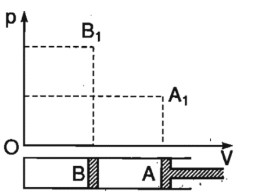
\includegraphics[width=0.35\linewidth]{figs/VN12-Y24-PH-SYL-015P-3}
	\end{center}
	\begin{enumerate}[label=(\arabic*)]
		\item Đẩy rất chậm từ A đến B.
		\item Đẩy rất nhanh từ A đến B rồi chờ cho trạng thái khí ổn định.
	\end{enumerate}
	Cho biết công nén trong quá trình nào lớn hơn?
	
	\choice
	{Cách 1}
	{\True Cách 2}
	{Hai cách như nhau}
	{Không thể kết luận được}
	\loigiai{\begin{itemize}
			\item \textbf{Cách 1:} Do nén chậm nên nhiệt độ khí không đổi. Lúc này công khí nhận bằng độ biến thiên nội năng:
			$$A_1=\Delta U.$$
			\item \textbf{Cách 2:} Nén nhanh khi nên nhiệt độ khí tăng nhanh (do không kịp toả nhiệt) nên công khí nhận vừa làm tăng nội năng khí vừa làm cho khí nóng lên.
			$$A_2=\Delta U+Q.$$
		\end{itemize}
	}
\end{ex}
% ===================================================================
\begin{ex}
	Độ biến thiên nội năng của khối khí lí tưởng đơn nguyên tử từ trạng thái $V_1=\SI{10}{\liter}$ và $p_1=\SI{1.5E5}{\pascal}$ đến trạng thái $V_2=\SI{20}{\liter}$ và $p_2=\SI{0.5E5}{\pascal}$ là
	
	\choice
	{$\Delta U=\SI{1150}{\joule}$}
	{\True $\Delta U=\SI{-750}{\joule}$}
	{$\Delta U=\SI{-1150}{\joule}$}
	{$\Delta U=\SI{750}{\joule}$}
	\loigiai{$$\Delta U=\dfrac{3}{2}\nu R\left(T_2-T_1\right)=\dfrac{3}{2}\left(p_2V_2-p_1V_1\right)=\SI{-750}{\joule}.$$
	}
\end{ex}
% ===================================================================
\begin{ex}
	Một cylanh thẳng đứng tiết diện $\SI{100}{\centi\meter^2}$ chứa khí ở nhiệt độ $\SI{27}{\celsius}$, phía trên được đậy bằng piston kín và cách nhiệt. Piston nhẹ, phía trên có đặt một vật nặng khối lượng $\SI{100}{\kilogram}$ và ban đầu cách đáy $\SI{60}{\centi\meter}$. Đốt nóng cylanh một cách từ từ để nhiệt độ khí tăng thêm $\SI{50}{\celsius}$. Cho áp suất khí quyển là $\SI{1.01E5}{\pascal}$, $g=\SI{9.8}{\meter/\second^2}$. Công do khí thực hiện là 
	
	\choice
	{$\SI{102}{\joule}$}
	{\True $\SI{199}{\joule}$}
	{$\SI{1200}{\joule}$}
	{$\SI{98}{\joule}$}
	\loigiai{Áp suất khí bên trong cylanh:
		$$p=p_0+\dfrac{mg}{S}=\SI{199E3}{\pascal}.$$
		Thể tích ban đầu của khí:
		$$V_1=Sh_1=\SI{6E3}{\centi\meter^3}.$$
		Đun từ từ nên áp suất khí trong cylanh không thay đổi:
		$$\dfrac{V_1}{T_1}=\dfrac{V_2}{T_2}\Rightarrow V_2=\SI{7E3}{\centi\meter^3}.$$
		Công do khí thực hiện:
		$$A'=p\left(V_2-V_1\right)=\SI{199}{\joule}.$$
	}
\end{ex}
% ===================================================================
\begin{ex}
Cho $\SI{1}{\mole}$ khí lí tưởng, khí thực hiện chu trình biến đổi trạng thái  $1-2-3-4-1$ như đồ thị trong hệ toạ độ $OVp$ ở hình bên. Các trạng thái 1 và 3 nằm trên cùng đường đẳng nhiệt. Nhiệt độ trạng thái 4 là $T_4=\SI{300}{\kelvin}$ và nhiệt độ ở trạng thái 2 là $T_2=\SI{390}{\kelvin}$. Công của khí nhận trên cả chu trình \textbf{gần nhất} với giá trị nào sau đây?
\begin{center}
	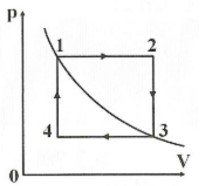
\includegraphics[width=0.3\linewidth]{figs/VN12-Y24-PH-SYL-015P-5}
\end{center}
	
	\choice
	{\True $\SI{50}{\joule}$}
	{$\SI{60}{\joule}$}
	{$\SI{70}{\joule}$}
	{$\SI{30}{\joule}$}
	\loigiai{\begin{center}
			\begin{tabular}{|C{3cm}|C{3cm}|C{3cm}|C{3cm}|}
				\hline
				\thead{Trạng thái} & $p$ & $V$ & $T$\\
				\hline
				1 & $p_1$ & $V_1$ & $T$\\
				\hline
				2 & $p_1$ & $V_3$ & $\SI{390}{\kelvin}$\\
				\hline
				3 & $p_3$ & $V_3$ & $T$\\
				\hline
				4 & $p_3$ & $V_1$ & $\SI{300}{\kelvin}$\\
				\hline
			\end{tabular}
		\end{center}
		$$\dfrac{pV}{T}=\text{const}\Rightarrow \dfrac{p_1V_1}{T_1}=\dfrac{p_1V_3}{390}=\dfrac{p_3V_3}{T}=\dfrac{p_3V_1}{300}=R\Rightarrow \begin{cases}
			p_1V_3=390R\\
			p_1V_1=p_3V_3=RT\\
			p_3V_1=300R
		\end{cases}\Rightarrow T=\sqrt{390\cdot300}=\xsi{30\sqrt{130}}{\kelvin}.$$
		Công của chu trình:
		$$A=\left(p_1-p_3\right)\left(V_3-V_1\right)=p_1V_3-p_1V_1-p_3V_3+p_3V_1=\left(390-30\sqrt{130}-30\sqrt{130}+300\right)R\approx\SI{49}{\joule}.$$
	}
\end{ex}
\Closesolutionfile{ans}
\subsection{TRẮC NGHIỆM ĐÚNG/SAI}
\setcounter{ex}{0}
% ===================================================================
\begin{ex}
	Một khối khí có thể tích $V_1=\SI{4}{\liter}$, áp suất $p=\SI{2E5}{\pascal}$ và nhiệt độ $t_1=\SI{57}{\celsius}$. Người ta thực hiện công $\SI{40}{\joule}$ để nén đẳng áp khối khí.
	\begin{enumerate}[label=\alph*)]
		\item Đồ thị biểu diễn quá trình nén khí trong hệ toạ độ $OpV$ là đoạn thẳng song song trục $OV$.
		\item Thể tích của khí sau khi nén bằng $\SI{3.8}{\liter}$.
		\item Nhiệt độ của khối khí sau khi nén bằng $\SI{313.5}{\celsius}$.
		\item Trong quá trình nén khí, khí toả nhiệt cho bên ngoài.
	\end{enumerate}
	\loigiai{\begin{enumerate}[label=\alph*)]
			\item Đúng.
			\item Đúng.
			$$A'=p\left(V_2-V_1\right)=\SI{-40}{\joule}\Rightarrow V_2=\SI{3.8E-3}{\meter^3}.$$
			\item Sai.\\
			$$\dfrac{V_1}{T_1}=\dfrac{V_2}{T_2}\Rightarrow T_2=\SI{313.5}{\kelvin}.$$
			\item Đúng. Vì $\Delta T<0$.
		\end{enumerate}
	}
\end{ex}
% ===================================================================
\begin{ex}
	Một khối khí lí tưởng có áp suất $p_1=\SI{3E3}{\pascal}$, thể tích $V_1=\SI{5}{\liter}$, nhiệt độ $t_1=\SI{27}{\celsius}$ được đun nóng đẳng áp đến nhiệt độ $t_2=\SI{177}{\celsius}$.
	\begin{enumerate}[label=\alph*)]
		\item Trong quá trình đun, khối khí thực hiện công.
		\item Thể tích lúc sau của khối khí là $\SI{32.7}{\liter}$.
		\item Công mà khối khí thực hiện có độ lớn bằng $\SI{7.5}{\joule}$.
		\item Nếu nhiệt lượng mà khí nhận được là $\SI{18.75}{\joule}$ thì độ biến thiên nội năng của khí là $\SI{26.25}{\joule}$. 
	\end{enumerate}
	
	\loigiai{\begin{enumerate}[label=\alph*)]
			\item Đúng.
			\item Sai.
			$$\dfrac{V_1}{T_1}=\dfrac{V_2}{T_2}\Rightarrow V_2=\SI{7.5}{\liter}.$$
			\item Đúng.
			$$A'=p\left(V_2-V_1\right)=\SI{7.5}{\joule}.$$
			\item Sai.
			$$\Delta U=Q+A=\SI{18.75}{\joule}-\SI{7.5}{\joule}=\SI{11.25}{\joule}.$$
		\end{enumerate}
	}
\end{ex}
% ===================================================================
\begin{ex}
\immini{
Một chiếc xe vượt qua sa mạc Sahara. Chuyến đi bắt đầu vào sáng sớm khi nhiệt độ là $\SI{3.0}{\celsius}$. Thể tích khí chứa trong mỗi lốp xe là $\SI{1.5}{\meter^3}$ và áp suất trong các lốp xe là $\SI{3.42E5}{\pascal}$. Coi khí trong lốp xe có nhiệt độ bằng nhiệt độ ngoài trời, không thoát ra ngoài và thể tích lốp không thay đổi. Đến giữa trưa, nhiệt độ tăng lên đến $\SI{42}{\celsius}$.

}	
{

\includegraphics[scale=0.2]{figs/VN12-Y24-PH-SYL-015P-2}
}
\begin{enumerate}[label=\alph*)]
	\item  Trong mỗi lốp xe có $\SI{164}{\mole}$ khí.
	\item Tốc độ căn quân phương của khí bên trong lốp xe vào giữa trưa tăng lên 1,07 lần so với lúc sáng sớm.
	\item Khi đến giữa trưa, áp suất khí trong lốp xe là $\SI{3.9E5}{\pascal}$.
	\item Từ sáng đến giữa trưa, động năng tịnh tiến trung bình của một phân tử khí trong lốp xe tăng $\SI{9.5E-21}{\joule}$.
\end{enumerate}

	\loigiai{\begin{enumerate}[label=\alph*)]
			\item  Sai.\\
			$$\nu=\dfrac{p_1V_1}{RT_1}\approx\SI{224}{\mole}.$$
			\item Đúng.
			$$\sqrt{\overline{v^2}}=\sqrt{\dfrac{3RT}{\mu}}\Rightarrow \dfrac{\sqrt{\overline{v^2_2}}}{\overline{v^2_1}}=\sqrt{\dfrac{T_2}{T_1}}=1,07.$$
			\item Đúng.
			$$\dfrac{p_2}{T_2}=\dfrac{p_1}{T_1}\Rightarrow p_2\approx\SI{3.9E5}{\pascal}.$$
			\item Sai.\\
			$$\Delta W_\text{đ}=\dfrac{3}{2}k\Delta T\approx\SI{8E-22}{\joule}.$$
		\end{enumerate}
	}
\end{ex}
% ===================================================================
\begin{ex}
	Khí helium đựng trong bình kín có thể tích $\SI{2}{\liter}$ ở nhiệt độ $\SI{27}{\celsius}$, áp suất $\SI{E5}{\pascal}$. Sau đó, người ta đung nóng khí trong bình đến nhiệt độ $\SI{127}{\celsius}$.
	\begin{enumerate}[label=\alph*)]
		\item Khối lượng riêng của khí helium ở nhiệt độ $\SI{27}{\celsius}$ là $\SI{160}{\kilogram/\meter^3}$.
		\item Tốc độ căn quân phương của mỗi nguyên tử khí ở trạng thái ban đầu là $\SI{1579}{\meter/\second}$.
		\item Trong quá trình đun nóng, khí không thực hiện công.
		\item Nhiệt lượng cung cấp để đun nóng khí trong điều kiện nói trên là $\SI{100}{\joule}$.
	\end{enumerate}
	
	\loigiai{\begin{enumerate}[label=\alph*)]
			\item Sai.
			$$\rho=\dfrac{p\mu}{RT}\approx\SI{0.16}{\kilogram/\meter^3}.$$
			\item Sai.
			$$\sqrt{\overline{v^2_1}}=\sqrt{\dfrac{3RT_1}{\mu}}\approx\SI{1368}{\meter/\second}.$$
			\item Đúng.
			\item Đúng. Vì $A=0$ nên
			$$Q=\Delta U=\dfrac{3}{2}\nu R\left(T_2-T_1\right)=\dfrac{3}{2}\cdot\dfrac{p_1V_1}{T_1}\cdot\left(T_2-T_1\right)=\SI{100}{\joule}.$$
		\end{enumerate}
	}
\end{ex}
% ===================================================================
\begin{ex}
	Một khối khí helium chứa trong bình có thể tích $\SI{5}{\liter}$, áp suất $\SI{1.5E5}{\newton/\meter^2}$. Nén đẳng áp khối khí để mật độ phân tử tăng gấp hai lần.
	\begin{enumerate}[label=\alph*)]
		\item Động năng trung bình của phân tử khí trước khi nén là $\SI{6.2E-11}{\joule}$.
		\item Mật độ phân tử khí trước khi nén là $\SI{3.6E-25}{\meter^{-3}}$.
		\item Nhiệt độ của khí sau khi nén là $\SI{150}{\celsius}$.
		\item Nhiệt lượng khí truyền cho bên ngoài là $\SI{562.5}{\joule}$.
	\end{enumerate}
	
	\loigiai{\begin{enumerate}[label=\alph*)]
			\item Đúng.
			$$W_\text{đ}=\dfrac{3}{2}kT\approx\SI{6.2E-21}{\joule}.$$
			\item Đúng.
			$$n=\dfrac{N}{V}=\dfrac{p}{kT}\approx\SI{3.6E25}{\meter^{-3}}.$$
			\item Sai.
			$$\dfrac{n_2}{n_1}=\dfrac{T_1}{T_2}\Rightarrow T_2=\SI{150}{\kelvin}\rightarrow t_2=\SI{-123}{\celsius}.$$
			\item Sai.
			$$Q=\Delta U+A'=\dfrac{3}{2}\nu R\left(T_2-T_1\right)+p\left(V_2-V_1\right)=\dfrac{5}{2}p\left(V_2-V_1\right)=\SI{-937.5}{\joule}.$$
		\end{enumerate}
	}
\end{ex}
\subsection{BÀI TẬP TỰ LUẬN}
\setcounter{ex}{0}
% ===================================================================
\begin{ex}
	Ở nhiệt độ phòng và áp suất $\SI{E5}{\pascal}$, không khí có khối lượng riêng khoảng $\SI{1.29}{\kilogram/\meter^3}$. Xác định giá trị trung bình của bình phương tốc độ các phân tử khí.
	\loigiai{$$p=\dfrac{1}{3}\rho \overline{v^2}\Rightarrow \overline{v^2}\approx\SI{23E4}{\meter^2/\second^2}.$$	}
\end{ex}
% ===================================================================
\begin{ex}
	Để động năng tịnh tiến trung bình của các phân tử khí bằng $\SI{1.0}{\electronvolt}$ thì nhiệt độ của khối khí phải bằng bao nhiêu $\si{\kelvin}$? Lấy $\SI{1}{\electronvolt}=\SI{1.6E-19}{\joule}$.
	
	\loigiai{$$W_\text{đ}=\dfrac{3}{2}kT\Rightarrow T\approx\SI{7729}{\kelvin}.$$
	}
\end{ex}
% ===================================================================
\begin{ex}
	Một bình dung tích $\SI{7.5}{\liter}$ chứa $\SI{24}{\gram}$ khí oxygen ở áp suất $\SI{2.5E5}{\newton/\meter^2}$. Tính động năng tịnh tiến trung bình của mỗi phân tử khí oxygen.
	
	\loigiai{$$W_\text{đ}=\dfrac{3}{2}kT=\dfrac{3}{2}\cdot\dfrac{RT}{N_A}=\dfrac{3}{2}\cdot\dfrac{M pV}{mN_A}\approx\SI{6.23E-21}{\joule}.$$
	}
\end{ex}
% ===================================================================
\begin{ex}
	Tính trung bình của bình phương tốc độ trong chuyển động nhiệt của phân tử khí helium có khối lượng mol là $\SI{4}{\gram/\mole}$ ở nhiệt độ $\SI{320}{\kelvin}$.
	
	\loigiai{$$W_\text{đ}=\dfrac{1}{2}m\overline{v^2}=\dfrac{3}{2}\cdot\dfrac{RT}{N_A}\Leftrightarrow \dfrac{1}{2}\cdot\dfrac{M}{N_A}\cdot\overline{v^2}=\dfrac{3}{2}\cdot\dfrac{RT}{N_A}\Rightarrow \overline{v^2}=\dfrac{3RT}{M}\approx\SI{2E6}{\meter^2/\second^2}.$$
	}
\end{ex}
% ===================================================================
\begin{ex}
	Xét khối khí trong bình kín, biết mật độ động năng phân tử (tổng động năng tịnh tiến trung bình của các phân tử khí trong $\SI{1}{\meter^3}$ khí) có giá trị $\SI{E-4}{\joule/\meter^3}$. Tính áp suất khí trong bình.
	\loigiai{$$\omega_\text{đ}=\dfrac{\sum W_\text{đ}}{V}=\dfrac{3}{2}\cdot\dfrac{n RT}{V}=\dfrac{3}{2}p\Rightarrow p=\dfrac{2}{3}\omega_\text{đ}\approx\SI{6.67E-5}{\pascal}.$$
	}
\end{ex}
% ===================================================================
\begin{ex}
	Bình thể tích $\SI{10}{\liter}$ chứa khí đơn nguyên tử có mật độ $\mu=\SI{3E-24}{\meter^{-3}}$. Động năng trung bình của nguyên tử là $\SI{5E-21}{\joule}$. Nội năng của khí trong bình bằng bao nhiêu?
	
	\loigiai{$$\mu=\dfrac{N}{V}\Rightarrow N=\mu V.$$
		Nội năng của khí:
		$$U=NW_\text{đ}=\mu V W_\text{đ}=\SI{150}{\joule}.$$
	}
\end{ex}
% ===================================================================
\begin{ex}
	Cho $\SI{20}{\gram}$ khí oxygen ở áp suất $\SI{2E5}{\newton/\meter^2}$, nhiệt độ $\SI{31}{\celsius}$ được đun nóng đẳng áp và dãn nở đến thể tích $\SI{25}{\liter}$. Công mà khí thực hiện trong quá trình trên bằng bao nhiêu?
	\loigiai{$$p_1V_1=\dfrac{m}{M}RT_1\Rightarrow V_1\approx\SI{7.9E-3}{\meter^3}.$$
		Công khí thực hiện:
		$$A'=p\left(V_2-V_1\right)\approx\SI{3.4}{\kilo\joule}.$$
	}
\end{ex}
% ===================================================================
\begin{ex}
	Cho $\SI{12}{\gram}$ khí hydrogen dãn nở đẳng áp, thể tích tăng gấp ba lần và thực hiện công $\SI{29916}{\joule}$. Nhiệt độ ban đầu của khí bằng bao nhiêu?
	
	\loigiai{Số mol khí:
		$$n=\dfrac{m}{M}=\SI{6}{\mole}.$$
		Qúa trình đẳng áp:
		$$\dfrac{V_2}{T_2}=\dfrac{V_1}{T_1}\Rightarrow T_2=3T_1\Rightarrow \Delta T=2T_1.$$
		Nhiệt độ ban đầu của khí:
		$$A'=n R\Delta T=2n RT_1\Rightarrow T_1\approx\SI{300}{\kelvin}.$$
	}
\end{ex}

% ===================================================================
\begin{ex}
	Một chất khí mà các phân tử có tốc độ căn quân phương là $\SI{1760}{\meter/\second}$ ở $\SI{0}{\celsius}$ thì tốc độ căn quân phương của các phân tử khí này ở nhiệt độ $\SI{1000}{\celsius}$ sẽ khoảng bao nhiêu?
	
	\loigiai{$$p=\dfrac{1}{3}\mu m\overline{v^2}=\dfrac{1}{3}\cdot\dfrac{Nm\overline{v^2}}{V}\Rightarrow pV=\dfrac{\sum m \overline{v^2}}{3}.$$
		Mà $pV=\dfrac{\sum m}{M}RT$.\\
		Như vậy:
		$$\overline{v^2}=\dfrac{3RT}{M}.$$
		Vì $\sqrt{\overline{v^2}}\sim \sqrt{T}$ nên:
		$$\sqrt{\overline{v^2_2}}=\sqrt{\overline{v^2_1}}\cdot\sqrt{\dfrac{T_2}{T_1}}\approx\SI{3.8E3}{\meter/\second}.$$
	}
\end{ex}
% ===================================================================
\begin{ex}
	Khối lượng phân tử khí hydrogen là $\SI{3.3E-24}{\gram}$. Biết rằng trong $\SI{1}{\second}$ có $\SI{E23}{}$ phân tử $\ce{H_2}$ với vận tốc $\SI{1000}{\meter/\second}$ đập vào $\SI{1}{\centi\meter^2}$ thành bình theo phương nghiêng $\SI{30}{\degree}$ so với thành bình. Áp suất khí lên thành bình bằng bao nhiêu?
	
	\loigiai{\begin{center}
			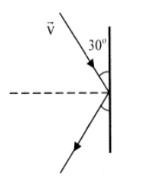
\includegraphics[width=0.2\linewidth]{figs/VN12-Y24-PH-SYL-015P-1}
		\end{center}
		Xét 1 phân tử khí $\ce{H_2}$:
		$$\Delta \vec{p}=\vec{f}\Delta t\Rightarrow 2mv\sin\alpha=p_1S\Delta t\Rightarrow p_1=\dfrac{2mv\sin\alpha}{S\Delta t}.$$
		Áp suất do khí $\ce{H_2}$ tác dụng lên thành bình:
		$$p=Np_1=\dfrac{2Nmv\sin\alpha}{S\Delta t}=\SI{3300}{\newton/\meter^2}.$$
	}
\end{ex}
% ===================================================================
\begin{ex}
	Một lượng khí thực hiện chu trình biến đổi trạng thái như hình bên. Cho biết: $t_1=\SI{27}{\celsius}$; $V_1=\SI{5}{\liter}$; $t_3=\SI{127}{\celsius}$; $V_3=\SI{6}{\liter}$. Ở điều kiện tiêu chuẩn, khí có thể tích $V_0=\SI{8.19}{\liter}$. Công do khí thực hiện sau một chu trình biến đổi trạng thái bằng bao nhiêu?
	\begin{center}
		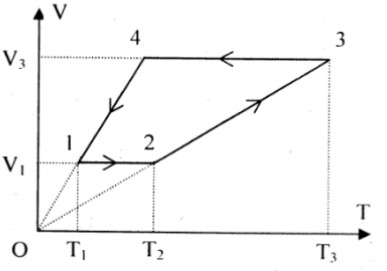
\includegraphics[width=0.35\linewidth]{figs/VN12-Y24-PH-SYL-015P-4}
	\end{center}
	
	\loigiai{\begin{center}
			\begin{tabular}{|C{3cm}|C{3cm}|C{3cm}|C{3cm}|}
				\hline
				\thead{Trạng thái} & $p$ & $V$ & $T$\\
				\hline
				0 & $\SI{101325}{\pascal}$ & $\SI{8.19}{\liter}$ & $\SI{273}{\kelvin}$\\
				\hline
				1 & $p_1$ & $\SI{5}{\liter}$ & $\SI{300}{\kelvin}$\\
				\hline
				2 & $p_2$ & $\SI{5}{\liter}$ & \\
				\hline
				3 & $p_2$ & $\SI{6}{\liter}$ & $\SI{400}{\kelvin}$\\
				\hline
				4 & $p_1$ & $\SI{6}{\liter}$ & \\
				\hline
			\end{tabular}
		\end{center}
		$$\dfrac{pV}{T}=\text{const}\Rightarrow \dfrac{p_0V_0}{T_0}=\dfrac{p_2V_3}{T_3}\Rightarrow p_2=\SI{182385}{\pascal}.$$
		Công do khí thực hiện trong chu trình là ở quá trình đẳng áp 2-3:
		$$A_{23}=p_2\left(V_3-V_2\right)=\SI{182.385}{\joule}.$$
	}
\end{ex}